\section{Collaborative ML Workload Optimizations} \label{sec-ml-workloads}
In this section, we provide an overview of our collaborative ML workload optimization system.
Figure \ref{system-workflow} shows the high-level architecture of our system.
Similar to collaborative environments, our system also comprises of a client and server component.
The client is responsible for parsing the user workload into a DAG (Step 1) and pruning the workload DAG (Step 2).
The server receives the workload DAG and utilizes our reuse algorithm to optimize the DAG (Step 3) and sends it back to the client.
Finally, the client executes the optimized DAG (Step 4) and prompts the server to update the Experiment Graph and store the artifacts of the executed workload DAG (Step 5).
This architecture enables us to integrate our system into the existing collaborative environments without requiring any changes to their workflow.
Similar to collaborative environments, the client and server can run within a single cloud environment where each client is an isolated container.
In the rest of this section, we describe the process of parsing, pruning, generating workload DAGs, and executing the workloads.
Then, we describe the process of constructing the Experiment Graph and how we utilize the Experiment Graph in our materialization and reuse algorithms. 
Finally, we show the integration process and the impact of our system on the use case in Section \ref{subsec-motivational-example}.

\begin{figure}
\centering
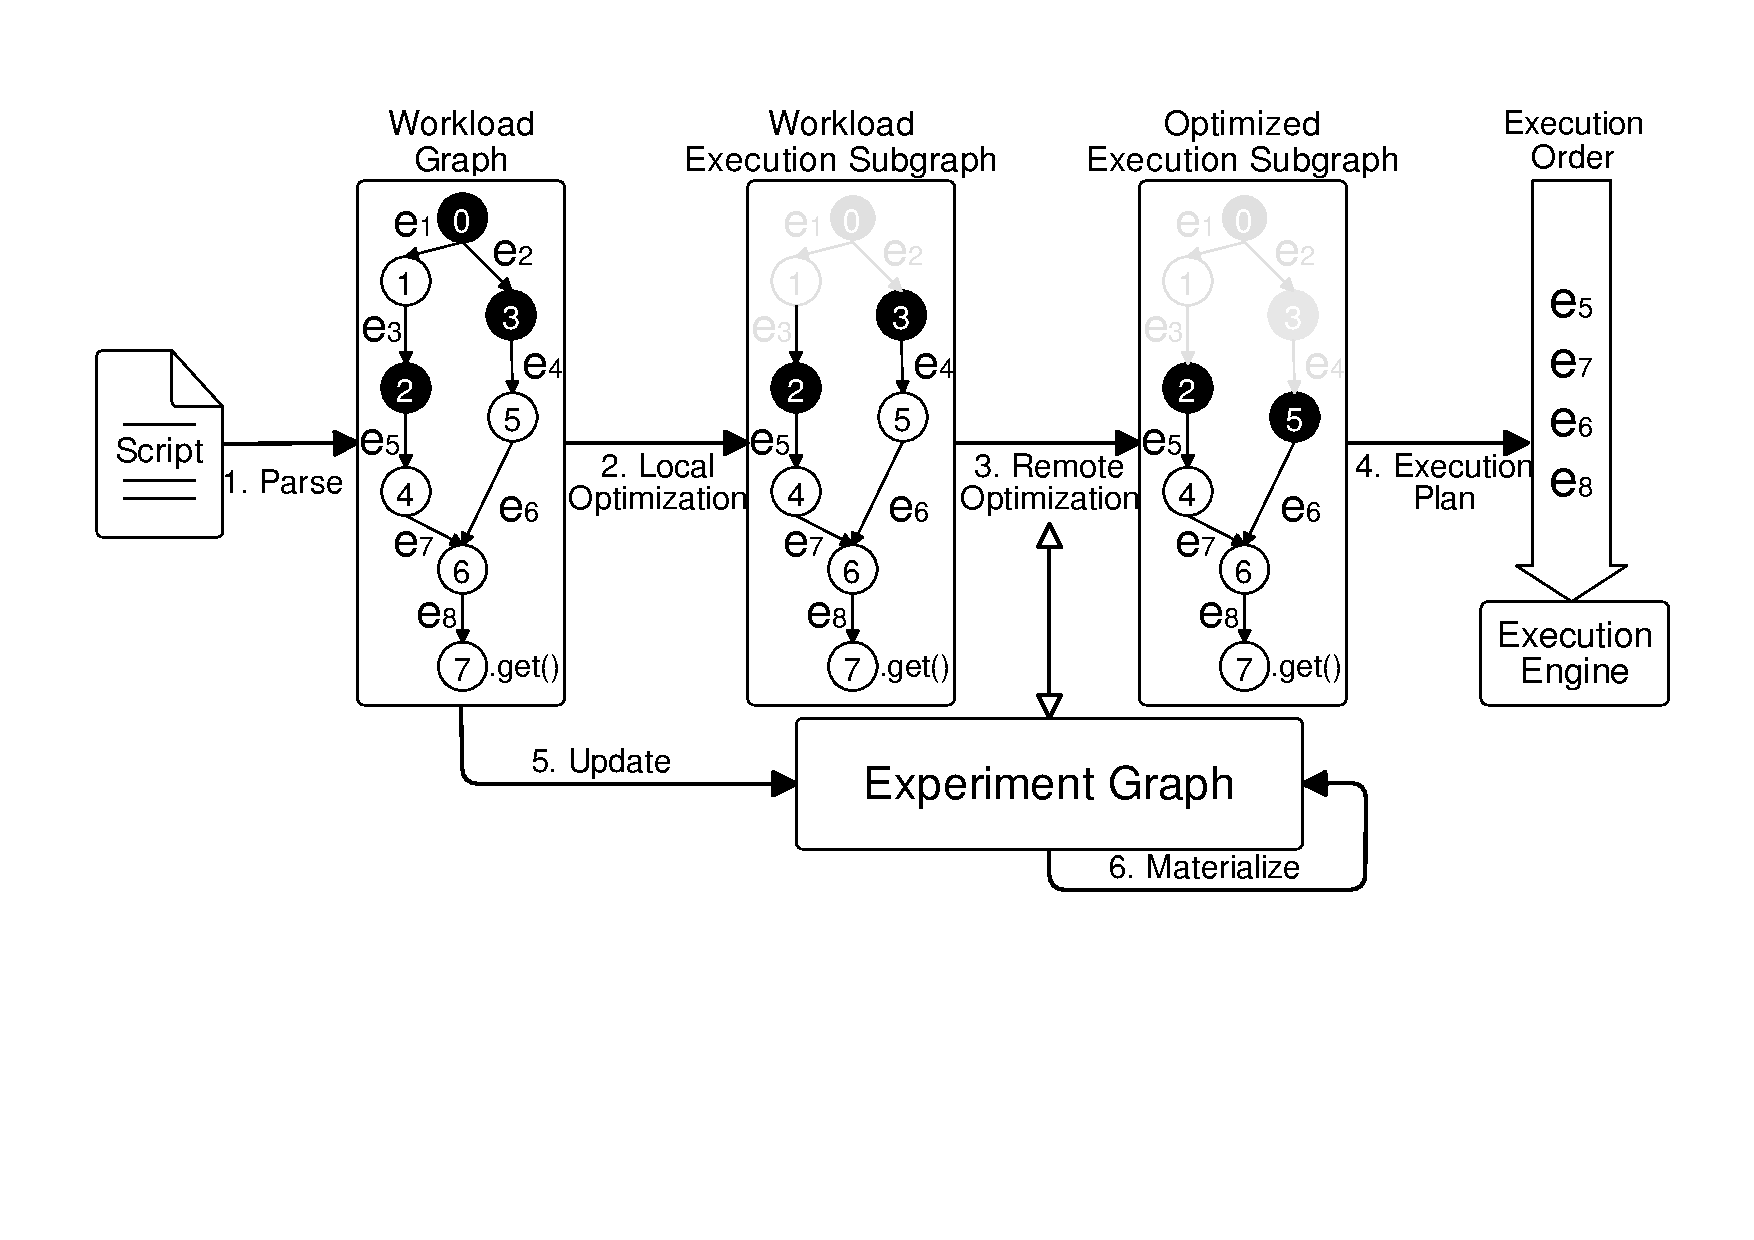
\includegraphics[width=0.9\columnwidth]{../images/system-workflow}
\caption{Overview of the collaborative workload optimizer system}
\label{system-workflow}
\end{figure}

\subsection{Client Components}
\textbf{ML Script and Parser.}
Instead of designing a new DSL, we extend the existing Pandas and scikit-learn \cite{sklearn_api} python packages that are common choices for data analysis and machine learning workloads.
Upon invocation of the program, the parser reads the script and transforms it into a DAG.
Listing \ref{listing-simple-workload} shows an example of a workload script.
The goal of the workload is to process a dataset of item descriptions, prices, and whether or not the items were purchased and train a classification model to predict whether new items will be purchased or not.
With only a slight modification of the import commands, we can load our parser modules.
As a result, we can support both long-running python scripts and interactive Jupyter notebooks.
\begin{lstlisting}[language=Python, caption=Example script,captionpos=b,label = {listing-simple-workload}]
import custom_pandas as pd

from custom_sklearn import svm
from custom_sklearn.feature_selection import SelectKBest
from custom_sklearn.feature_extraction.text import CountVectorizer

train = pd.read_csv('path-to-datasets/train.csv') 
print train.columns # [ad_desc,ts,u_id,price,y]
ad_desc = train['ad_desc']
vectorizer = CountVectorizer()
cnt_vect = vectorizer.fit_transform(ad_desc)
selector =  SelectKBest(k=2)
t_subset = train[['ts','u_id','price']]
y =  train['y']
top_feats = selector.fit_transform(
                                  t_subset,  
                                  y )
top_features # print the content of the data frame		     
X = pd.concat([count_vectorized,top_features], axis = 1)
model = svm.SVC().fit(X, train['y'])
print model # terminal vertex
\end{lstlisting}

\textbf{Workload DAG.}
In our DAG representation, vertices are the artifacts, i.e., raw or preprocessed data (represented by data frame objects) and machine learning models resulting from feature engineering and model training operations and edges are the operations in the workload.
Each workload DAG has one or more vertices representing the raw datasets.
We refer to such vertices as sources.
A workload DAG also contains one or more terminal vertices.
Terminal vertices represent the output of the workload.
For example, a terminal vertex is a trained ML model, a preprocessed dataset, or aggregated data for visualization.
Requesting the result of a terminal vertex triggers the optimization and execution of the workload DAG.
Figure \ref{fig-workload-dag} shows the workload DAG constructed from the code in Listing \ref{listing-simple-workload}.
In the Figure, the highlighted vertex represents a terminal vertex, which is the result of the print statement on Line 21 in Listing \ref{listing-simple-workload}.
\begin{figure}
\centering
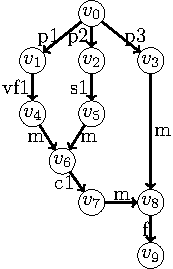
\includegraphics[width=\linewidth]{../images/tikz-standalone/example-graph}
\caption{Workload DAG constructed from the Listing \ref{listing-simple-workload}. The highlighted node shows a terminal vertex.}
\label{fig-workload-dag}
\end{figure}

\textbf{Local Pruner.}
Once the user requests the result of a terminal vertex, the client prunes the DAG before sending it to the server.
The task of the pruner is to identify all the unnecessary edges.
There are two groups of unnecessary edges: edges that are not in the path from source to terminal and edges with their endpoint vertex already computed.
The latter is very common in interactive workloads since every cell invocation in Jupyter notebooks computes some of the vertices.
As a result, in the future cell invocations, previously executed operations can be skipped.
Note that the pruner does not remove the unnecessary edges from the DAG and only marks them as inactive.
For example, in Figure \ref{fig-workload-dag}, if \textit{t\_subset} is previously computed, the local pruner marks the edge between \textit{train} and \textit{t\_subset} as inactive.
After the pruning, the client sends the DAG to the server.
To minimize the transfer cost, the client does not send the content of the computed artifact to the server.

\textbf{Executor. }
After the server optimizes a workload DAG, the executor receives the optimized DAG to execute the operations and returns the result to the user.
The executor runs the operations in the optimized DAG in their topological order and returns the result to the user.
To avoid redundant computation, the executor ignores inactive edges.
After the executor completes the execution of a workload DAG, it annotates the DAG vertices with compute-time and sizes before sending it to the updater for storage.

%
%\begin{figure}\label{DAG-workflow}
%\begin{subfigure}{\columnwidth}
%\centering
%\includegraphics[width=0.8\linewidth]{../images/tikz-standalone/system-workflow-legend}
%\end{subfigure}
%\begin{subfigure}{0.3\columnwidth}
%\centering
%\includegraphics[width=0.8\linewidth]{../images/tikz-standalone/system-workflow-1}
%\parbox{3cm}{\caption{Original DAG}}
%\end{subfigure}%
%\begin{subfigure}{0.3\columnwidth}
%\centering
%\includegraphics[width=0.8\linewidth]{../images/tikz-standalone/system-workflow-2}
%\parbox{3cm}{\caption{Pruned DAG}}
%\end{subfigure}%
%\begin{subfigure}{0.3\columnwidth}
%\centering
%\includegraphics[width=0.8\linewidth]{../images/tikz-standalone/system-workflow-3}
%\parbox{3cm}{\caption{Optimized DAG}}
%\end{subfigure}
%\label{fig-experiment-graph}
%\caption{Different stages of a Workload DAG. Loaded: an artifact with its underlying data available, Computed: an artifact who is previously computed in an interactive workload, Materialized: an artifact which is available in the Experiment Graph, Null: an artifact which is not yet computed}
%\end{figure}

\subsection{Server Components}
\textbf{Experiment Graph (EG).}
EG is the union of all the executed workload DAGs, where vertices represent the artifacts and edges represent the operations.
Every vertex in EG has the attributes $frequency$, $size$, and $compute\_time$, representing the number of different workloads an artifact appeared in, the storage size of the artifact, and the time required to compute the artifact given its input artifacts, respectively.
Every vertex in the experiment Graph carries the meta-data of the artifact it represents.
For datasets, the meta-data includes the name, type, and size of each column.
For ML models, the meta-data includes the name, type, hyperparameters, and the evaluation score of the model.
To save storage space, EG does not contain the underlying content, i.e., Pandas data frame and model weights, of all the artifacts.
The updater component decides whether to store the underlying content of an artifact.

EG maintains a list of all the source vertices that it contains.
Furthermore, every edge in the graph stores the hash of the operation it represents.
Therefore, given a workload DAG, the Experiment Graph can quickly detect if it contains any of the artifacts of the workload DAG by traversing the edges starting from the source.
%Note that we construct one EG per ML task.
%Every source vertex of EG corresponds to a training or testing dataset in the ML task.
%Furthermore, all the model artifacts in EG are evaluated using the metric defined in the ML task.
%As a result, we can compare ML model performances, which is a requirement for our materialization algorithm.

\textbf{Optimizer. }
The optimizer receives the workload DAG from the client and queries the Experiment Graph for materialized artifacts.
Then, the optimizer utilizes our reuse algorithm to generate an optimized DAG with some of its vertices already materialized.
Similar to the local pruning step, the optimizer also marks unnecessary edges as inactive before returning the optimized DAG to the client.
The optimized DAG guarantees to incur the smallest execution cost, i.e., the cost of transferring the materialized artifacts plus executing the remaining operations.

\textbf{Updater.}
The updater receives the executed DAG from the client.
The vertices in the executed DAG contain the size and compute-time of the artifacts they represent.
The updater performs the three following tasks.
First, it stores any source artifact, both the meta-data and the underlying content, that is not in EG.
This is to ensure that EG contains every raw dataset.
Second, it updates EG to include all the vertices and edges of the executed DAG.
If EG already contains a vertex, the updater increases its frequency.
Lastly, by utilizing our materialization algorithm, the updater stores the underlying content of a selected set of artifacts, i.e., the output of the materialization algorithms.
The materialization algorithms select the artifacts by considering their run-time, size, frequency, and score of ML models.
Note that the Experiment Graph contains the meta-data of all the artifacts, including the unmaterialized artifacts.

%Each edge contains the meta-data of the operation it represents, such as the function name, training algorithm, and hyperparameters.
%To uniquely identify an edge, we utilize a hash function which receives as input the operation and its hyperparameters (if it has any).
%Since the experiment graph is rooted, we assign a hash value to every vertex which is computed in the following way:
%\[
%    h(v)= 
%\begin{cases}
%    id,& \text{if } v \text{ is root}\\
%    h\Big(\sum\limits_{e \in in\_edge(v)} (h(e.source) + h(e) ) \Big)  ,              & \text{otherwise}.
%\end{cases}
%\]
%where $in\_edge(v)$ returns the edges with destination $v$. 
%Intuitively, the hash of a root vertex is its unique identifier (location on disk or download URL) and the hashes of other vertices are derived recursively by combining the hashes of their parents and edges which connect them to their parents.

%After a machine learning workload is executed, we update the experiment graph by adding the new artifacts and operations.
%If any of the artifacts already exist in the graph, their frequency is updated.
%We start with an empty Experiment Graph.
%After the execution of the script and updating the Experiment Graph, all the artifacts (vertices) have a frequency of 1.
%To represent operations which process multiple input artifacts, e.g., concat and svm.fit operations in Listing \ref{listing-experiment-graph}, we proceed as follows.
%First, we merge the vertices representing the artifacts into a single vertex using a merge operator.
%The merge operator is a logical operator which does not incur a cost, i.e., it has a run-time of 0 seconds.
%The merged vertex is also a logical vertex with no actual attributes which only contains the vertex ids of the merged vertices.
%Then, we draw an edge from the merged vertex which represents the actual operation.
%For example, in Figure \ref{fig-experiment-graph}a, before applying the concatenation operation, we merge $v_4$ and $v_5$ into $v_6$, then we apply the concatenation operation (c1).
%Furthermore, when computing the hash of a merged vertex, we take the merge order into account.
%For example, the operation svm.fit has $X$ (represented by $v_7$) as first argument and train['y'] (represented by $v_3$) as its second argument.
%When computing hash of $v_8$, we combine the parents in the same order, i.e., $h(v_8) = h(h(v_7) + m + h(v_3) + m)$. 
%After the DAG is constructed, its execution is invoked with the call to the $get()$ command on Line 18.
%\subsection{System Architecture and Workflow}
%Figure \ref{system-workflow} shows the components of our collaborative workload optimizer system.
%First, a parser component generates the workload DAG from the user scripts (Step 1).
%Upon the invocation of the $get()$ method of a vertex, i.e., the terminal vertex, a local optimization process beings.
%The local optimizer extracts the subgraph which must be executed in order to compute the terminal vertex.
%The local optimizer traverses the graph in reverse order starting at the terminal vertex until the root vertices.
%It stops the traversal when it reaches a previously computed vertex.
%In interactive workloads, it is likely that many of the intermediate vertices between the terminal vertex and the root vertices are previously computed.
%The subgraph of all the visited vertices and the edges connecting them is another DAG, which we refer to as the \textit{local execution DAG}, and is the result of the local optimizer (Step 2).
%The global optimizer component receives the local execution DAG and looks for optimization opportunities, i.e., reusing materialized vertices or warmstarting model training, in the experiment graph.
%Using early stopping, search space pruning, and heuristics the global optimizer finds the relevant artifacts \hl{with negligible overhead}.
%The result of the global optimization process is another subgraph, which we refer to as the \textit{global execution DAG} (Step 3).
%Then, an execution planner receives the global execution DAG and generates the execution schedule by sorting the edges based on their topological order, which is then executed by the execution engine (Step 4).
%If the experiment graph is empty, then the execution planner users local execution DAG to generate the execution schedule.
%After the execution, an updater component updates the experiment graph to include the vertices and edges of the workload DAG (Step 5).
%Lastly, a materializer component decides what vertices to materialize, i.e., store their underlying data in the vertex of the graph (Step 6).

\subsection{Improved Use Case}
In this section, we show how our collaborative workload optimizer improves the workload execution process of the Kaggle use case.
We maintain an Experiment Graph for the Home Credit Default Risk competition.
After users start publishing their workload scripts on the Kaggle platform, other users will read, re-run, or modify the existing scripts.
The updater component of our system stores the artifacts with a high likelihood of reuse into EG.
Our optimizer generates efficient workloads by querying EG for materialized artifacts and transforming the workload DAG into a more optimized DAG.
In the use case, we highlighted 3 workloads that were copied and modified 7000 times.
Optimizing the execution of these workloads saves 100s of hours of execution time.
As a result, our collaborative optimizer reduces the required resources and operation cost of Kaggle.

